


\tikzset{every picture/.style={line width=0.75pt}} %set default line width to 0.75pt        

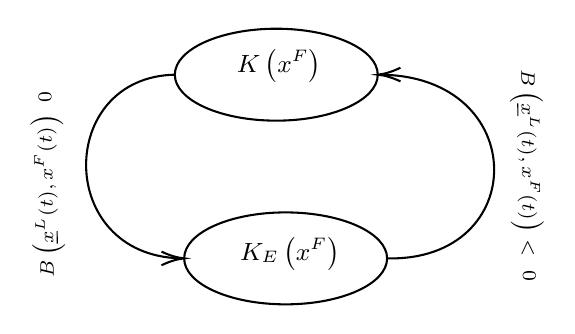
\begin{tikzpicture}[x=0.75pt,y=0.75pt,yscale=-1,xscale=1]
%uncomment if require: \path (0,300); %set diagram left start at 0, and has height of 300

%Shape: Ellipse [id:dp7990490888023698] 
\draw   (228.5,85.15) .. controls (228.5,72.92) and (250.39,63) .. (277.38,63) .. controls (304.38,63) and (326.27,72.92) .. (326.27,85.15) .. controls (326.27,97.38) and (304.38,107.3) .. (277.38,107.3) .. controls (250.39,107.3) and (228.5,97.38) .. (228.5,85.15) -- cycle ;
%Shape: Ellipse [id:dp4992846433905609] 
\draw   (233,173.65) .. controls (233,161.42) and (254.89,151.5) .. (281.88,151.5) .. controls (308.88,151.5) and (330.77,161.42) .. (330.77,173.65) .. controls (330.77,185.88) and (308.88,195.8) .. (281.88,195.8) .. controls (254.89,195.8) and (233,185.88) .. (233,173.65) -- cycle ;
%Curve Lines [id:da3597348211087257] 
\draw    (330.77,173.65) .. controls (399.92,175.29) and (400.27,85.7) .. (327.37,85.15) ;
\draw [shift={(326.27,85.15)}, rotate = 359.73] [color={rgb, 255:red, 0; green, 0; blue, 0 }  ][line width=0.75]    (10.93,-3.29) .. controls (6.95,-1.4) and (3.31,-0.3) .. (0,0) .. controls (3.31,0.3) and (6.95,1.4) .. (10.93,3.29)   ;
%Curve Lines [id:da038428937296795196] 
\draw    (228.5,85.15) .. controls (171.35,86.29) and (170.78,172.06) .. (231.15,173.63) ;
\draw [shift={(233,173.65)}, rotate = 179.86] [color={rgb, 255:red, 0; green, 0; blue, 0 }  ][line width=0.75]    (10.93,-3.29) .. controls (6.95,-1.4) and (3.31,-0.3) .. (0,0) .. controls (3.31,0.3) and (6.95,1.4) .. (10.93,3.29)   ;

% Text Node
\draw (256.91,71.5) node [anchor=north west][inner sep=0.75pt]  [font=\small]  {$K\left( x^{F}\right)$};
% Text Node
\draw (258.41,162) node [anchor=north west][inner sep=0.75pt]  [font=\small]  {$K_{E}\left( x^{F}\right)$};
% Text Node
\draw (407.28,80.97) node [anchor=north west][inner sep=0.75pt]  [font=\scriptsize,rotate=-89.52]  {$B\left(\underline{x}^{L}( t) ,x^{F}( t)\right) < \ 0$};
% Text Node
\draw (158.44,184.72) node [anchor=north west][inner sep=0.75pt]  [font=\scriptsize,rotate=-269.17]  {$B\left(\underline{x}^{L}( t) ,x^{F}( t)\right) \geqslant \ 0$};


\end{tikzpicture}
